\documentclass[12pt,letterpaper]{article}
\usepackage[spanish]{babel}
\usepackage[utf8]{inputenc}
\usepackage{graphicx}
\usepackage{pst-pdf}
\usepackage{amssymb}
\usepackage{hyperref}
\usepackage{listings}
\title{{Programacion estructurada.}}
\author{Daniel Reyes Barrera}
\date{2 de diciembre de 2020}

\begin{document}
\maketitle

\abstract{En este documento se han resuelto algunos problemas computacionales utilizando las herramientas aprendidas en la clase 6 – Punteros, arreglos, uso de memoria. del curso de programaci\'on C++, como son direcciones de memoria, punteros, memoria estatica y dinamica, arreglos y arreglos multidimencionales}



\section{Ejercicio 1.}

Hacer un mapa conceptual con los conceptos de esta clase: arreglos unidimensionales, multidimensionales, paso por referencia, paso por valor, memoria est\'atica, memoria din\'amica, etc.
\begin{figure}[ht!]
  \centering
  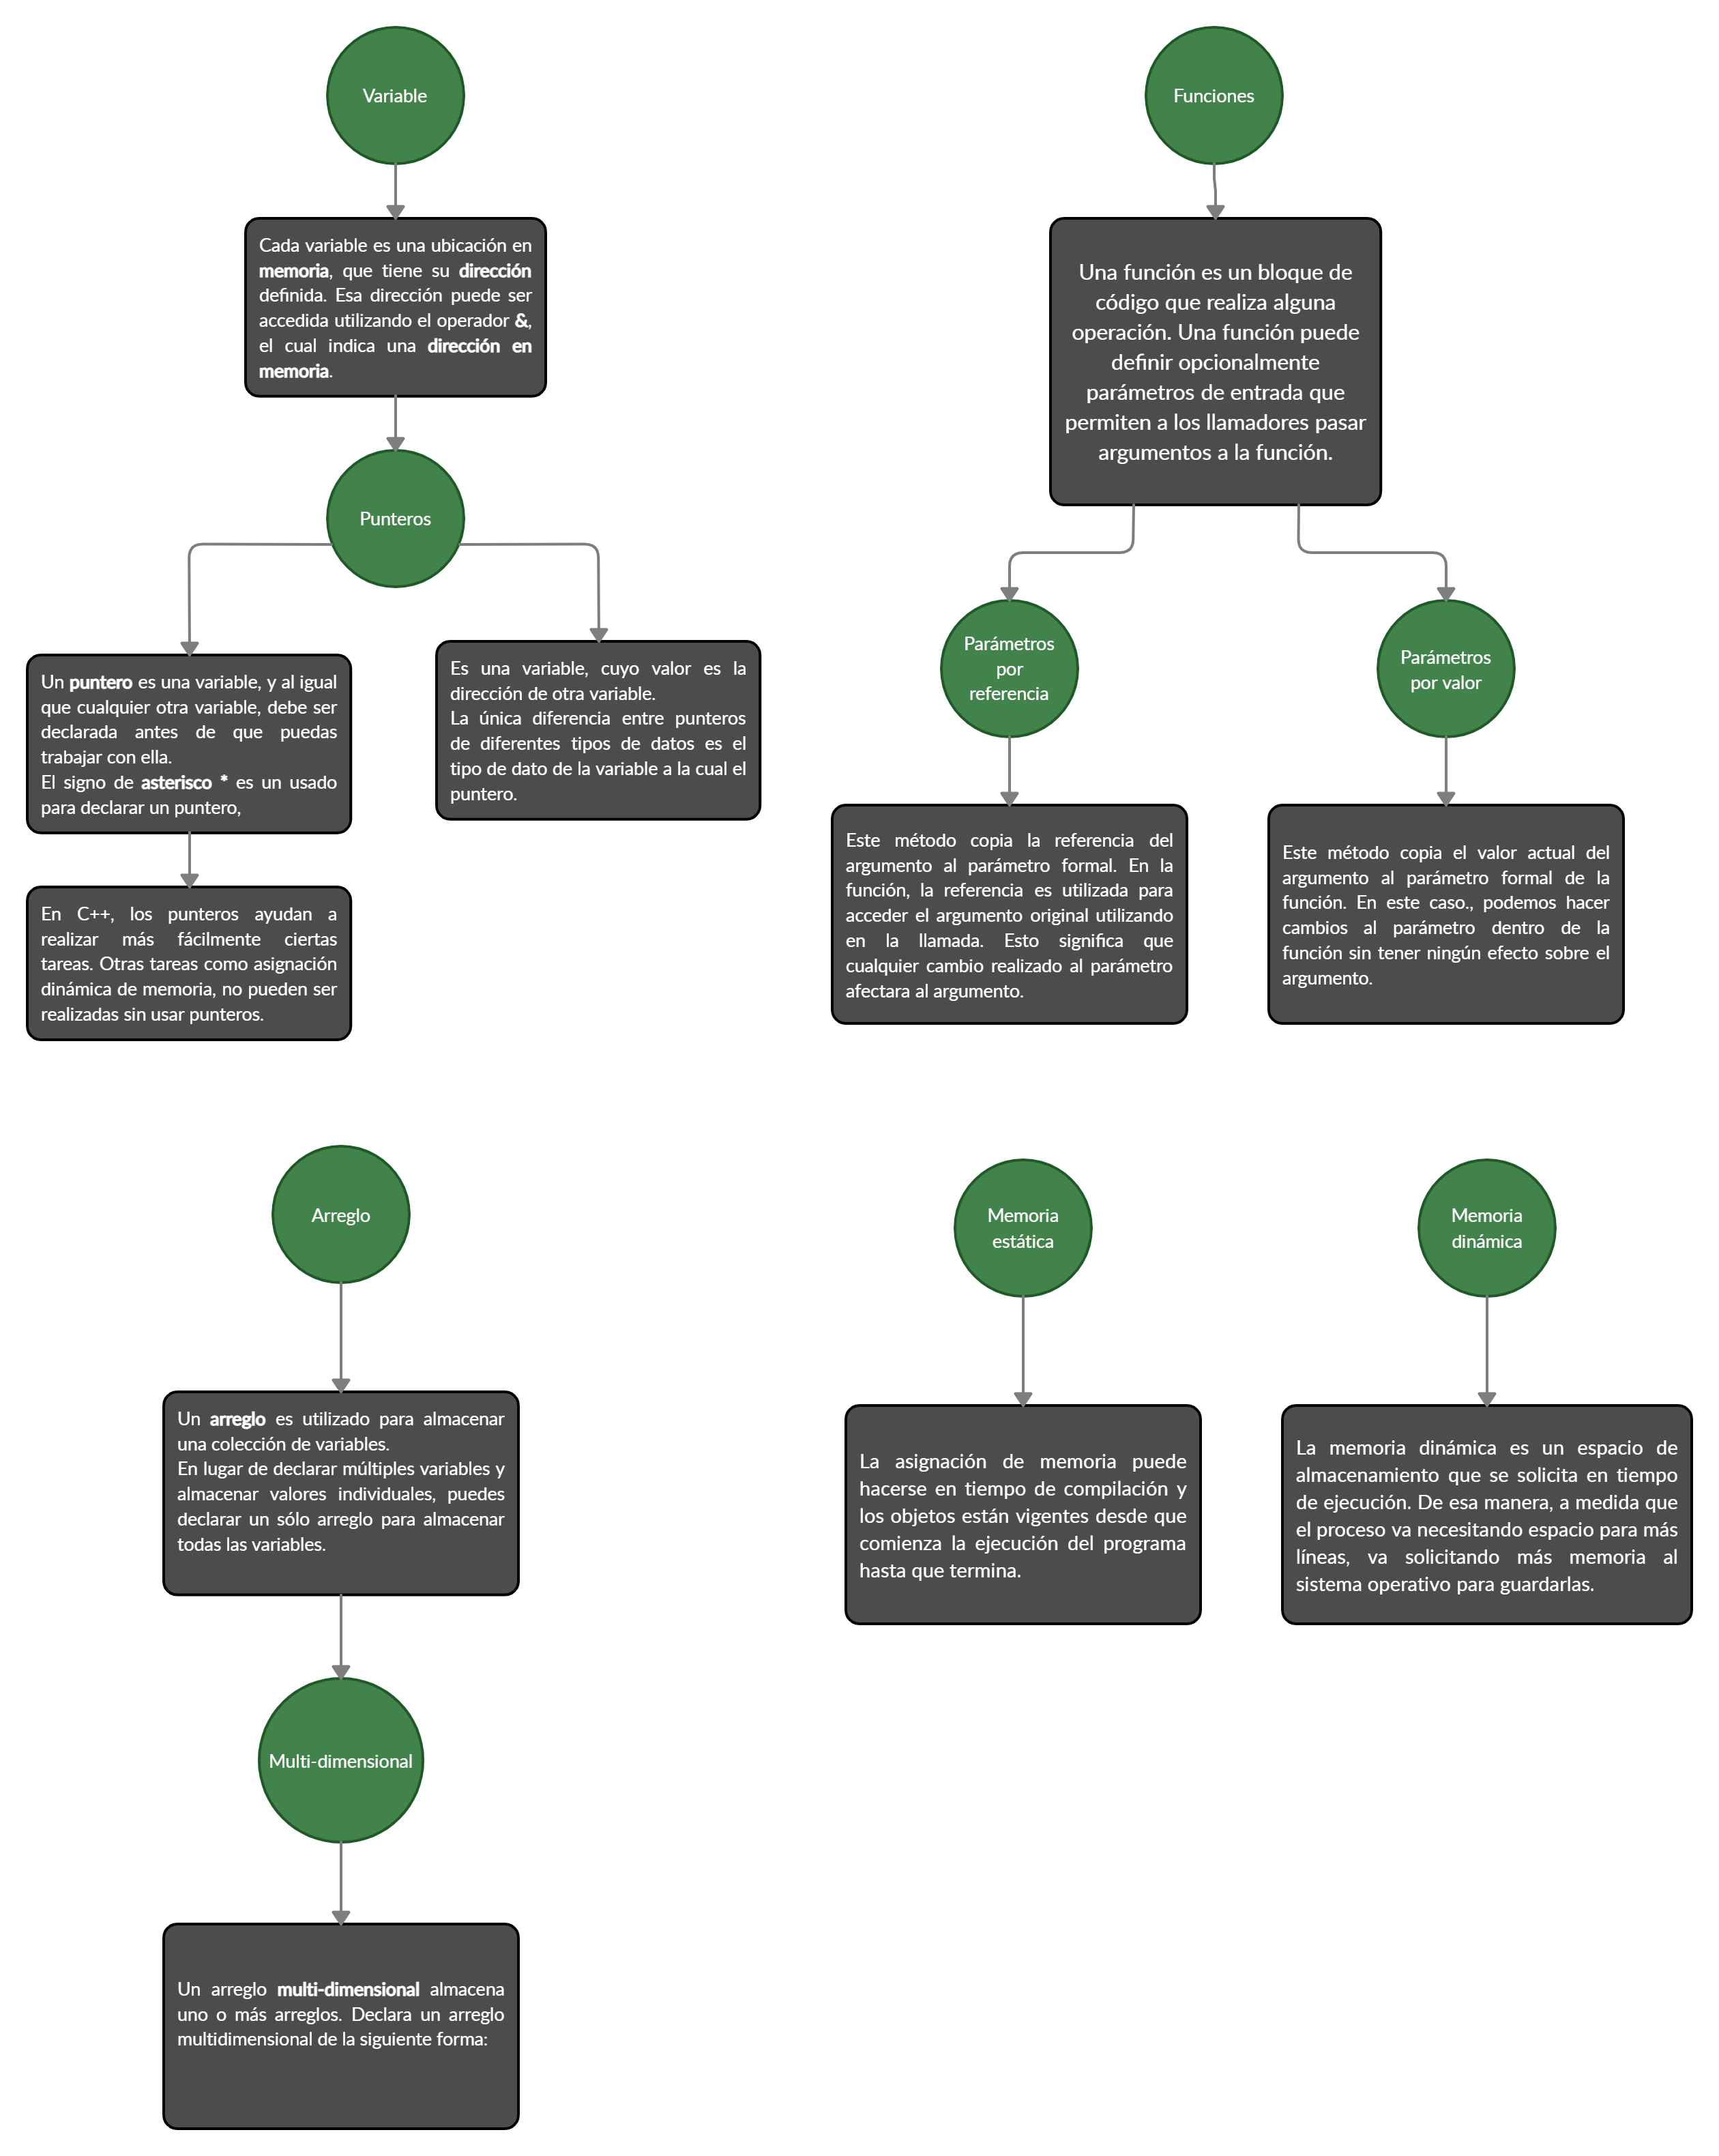
\includegraphics[width=1\textwidth]{figures/mapa}
  \caption{Mapa conceptual}
\end{figure}

\newpage

\section{Primer programa}
El m\'aximo com\'un divisor de dos enteros es el entero m\'as grande que puede dividir a cada uno de los dos n\'umeros. Programe el algoritmo para calcular el m\'aximo com\'un divisor en un m\'etodo independiente.

\subsection{Problema computacional.}
\textbf{Objetivo:} Dado dos n\'umero enteros calcular el m\'aximo comun divisor.

\textbf{Entrada:} Dos n\'umeros enteros.

\textbf{Salida:} El valor de MCD de ambos n\'umeros introducidos.

\subsection{Algoritmo.}
Se reutilizo el c\'odigo de la tarea 5 y se le hizo una modificaci\'on para utilizar punteros, especificamente el paso de par\'ametros por referencia como apuntadores.

El código fuente del programa se muestra en el Apéndice \ref{code:MCD}.
\subsection{Instancia del problema.}
Como prueba de escritorio, se seleccionaron las siguientes instancias del problema. Entrada: $a=45 $, $b=50$ y $a=1032$, $b=180$. La salida del programa se observa en la Figura \ref{fig:MCD}.
\begin{figure}[ht!]
  \centering
  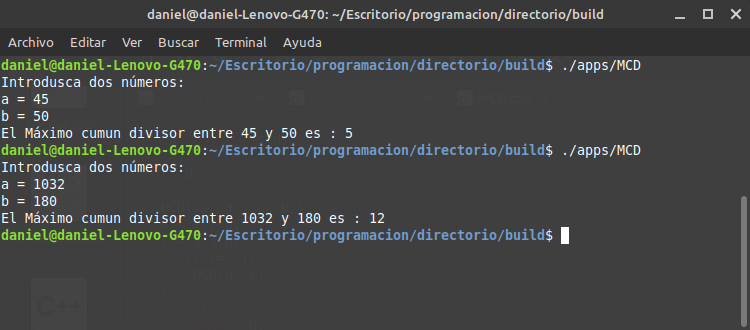
\includegraphics[width=0.8\textwidth]{figures/MCD}
  \caption{Ejecución de algunas instancias del problema.}
  \label{fig:MCD}
\end{figure}
\newpage

\section{Segundo programa}

Programe el algoritmo para determinar si el n\'umero es pal\'indromo y el algoritmo para validar la entrada en m\'etodos independientes.
Sugerencia: Haga uso de los operadores m\'odulo y divisi\'on para separar el n\'umero tecleado en unidades, decenas, centenas, etc.

Escriba un programa que imprima un men\'u para seleccionar un tipo de figura geom\'etrica de la siguiente forma:
\begin{figure}[ht!]
  \centering
  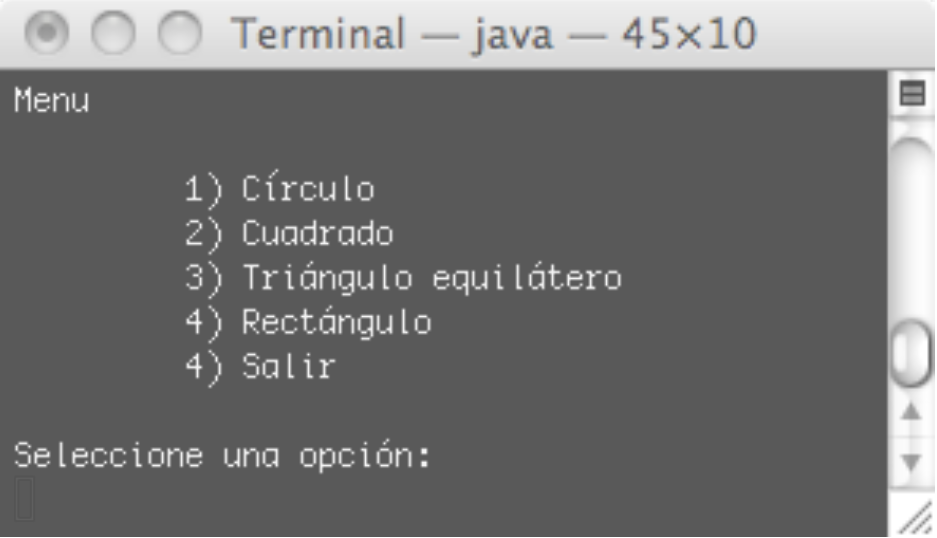
\includegraphics[width=0.6\textwidth]{figures/captura}
\end{figure}

El usuario debe seleccionar una opci\'on y el programa debe calcular el \'area y per\'imetro de la opci\'on seleccionada. Programe cada opci\'on en un m\'etodo independiente. El programa debe regresar al menu principal hasta que el usuario seleccione la opci\'on salir.

\subsection{Problema computacional.}
\textbf{Objetivo:} Calcular \'areas de figuras deseadas de manera indefinida.

\textbf{Entrada:} Un n\'umero que represente la figura deseada y posteriormente sus dimensiones.

\textbf{Salida:} El area de la figura deseada.

\subsection{Algoritmo.}
Se reutiliz\'o el codigo de la tarea 5, reescribiendolo talque se pasar\'a la variable de retorno por referencia.

El c\'odigo fuente del programa se muestra en el Apéndice \ref{code:calcular_area}.

\subsection{Instancia del problema.}
Como prueba de escritorio, se seleccionaron las siguientes instancias del problema.Se calcularon las siguientes \'areas: Un circulo de radio 4 y el \'area de un rectangulo de base = 2 y altura = 5. . La salida del programa se observa en la Figura \ref{fig:calcular_area}.
\begin{figure}[ht!]
  \centering
  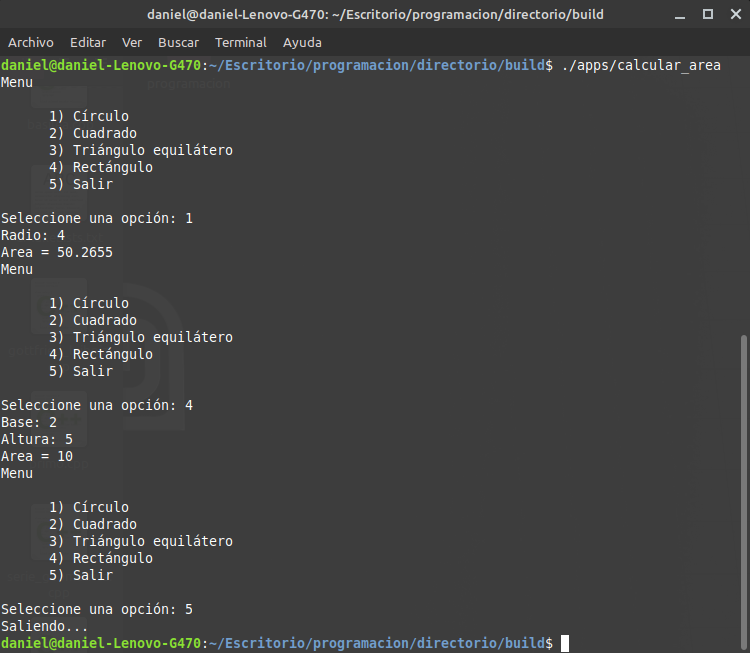
\includegraphics[width=0.8\textwidth]{figures/calcular_area}
  \caption{Ejecución de algunas instancias del problema.}
  \label{fig:calcular_area}
\end{figure}

\newpage

\section{Tercer programa}

Programe el algoritmo para determinar si el n\'umero es pal\'indromo y el algoritmo para validar la entrada en m\'etodos independientes.
Sugerencia: Haga uso de los operadores m\'odulo y divisi\'on para separar el n\'umero tecleado en unidades, decenas, centenas, etc.

\subsection{Problema computacional.}
\textbf{Objetivo:} Dado un n\'umero entero determinar si es pal\'indromo.

\textbf{Entrada:} Un n\'umero entero mayor que 0.

\textbf{Salida:} La respuesta de si el n\'umero dado es o no pal\'indromo.

\subsection{Algoritmo.}
En este se utiliz\'o el pasar la variable de retorno como apuntador.


El código fuente del programa se muestra en el Apéndice \ref{code:palindromo}.

\subsection{Instancia del problema.}
Como prueba de escritorio, se seleccionaron las siguientes instancias del problema. Entrada: 12344321, 2234321, 76567 y 12324. La salida del programa se observa en la Figura \ref{fig:palindromo}.
\begin{figure}[ht!]
  \centering
  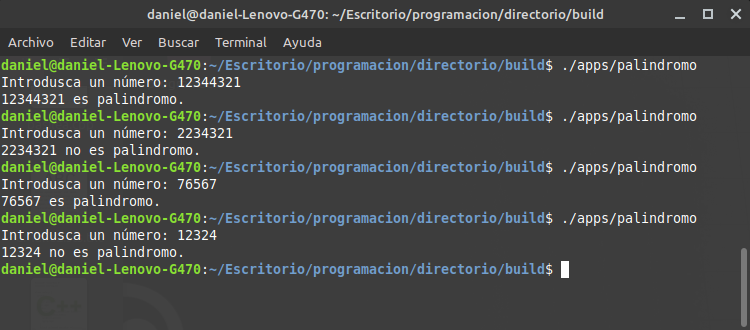
\includegraphics[width=0.8\textwidth]{figures/palindromo}
  \caption{Ejecución de algunas instancias del problema.}
  \label{fig:palindromo}
\end{figure}
\newpage

\section{Cuarto programa}

Escriba un programa que capture 15 n\'umeros y los imprima ordenados de menor a mayor.

\subsection{Problema computacional.}
\textbf{Objetivo:} Ordenar una cantidad de $n$ n\'umeros dados por el usuario.

\textbf{Entrada:} Una serie de n\'umeros.

\textbf{Salida:} Los n\'umeros dados por el usuario impresos de menor a mayor.

\subsection{Algoritmo.}
Se utiliz\'o un arreglo dinamico para el ordenamiento de los n\'umeros.


El código fuente del programa se muestra en el Apéndice \ref{code:ordenar_numeros}.

\subsection{Instancia del problema.}
Como prueba de escritorio, se seleccionó la siguiente instancia del problema. Entrada: 45, 2, 6, 23, 34, 87, 1, 0, 41, 24, 14, 19, 28, 9 y 10 . La salida del programa se observa en la Figura \ref{fig:ordenar_numeros}.
\begin{figure}[ht!]
  \centering
  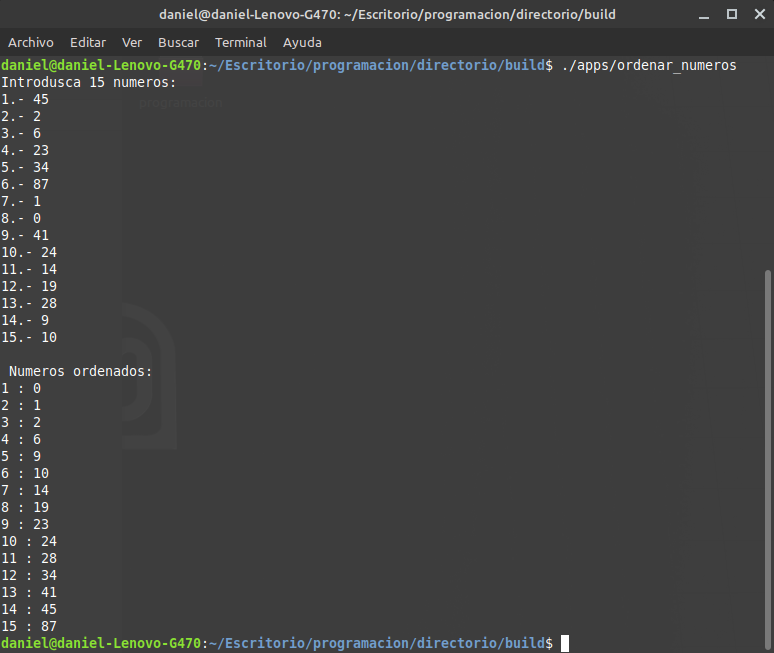
\includegraphics[width=0.8\textwidth]{figures/ordenar_numeros}
  \caption{Ejecución de algunas instancias del problema.}
  \label{fig:ordenar_numeros}
\end{figure}

\newpage

\section{Conclusiones.}

El programar con apuntadores y tener en cuenta la memoria estarica y dinamica tiene muchos beneficios cuando se programa un gran algoritmo. Otra de las grandes ventajas de la utilizaci\'on de punteros es la posibilidad de realizar una asiganaci\'on din\'amica de memoria. Esto significa que la reserva de memoria se realiza din\'amicamente en tiempo de ejecuci\'on, no siendo necesario entonces tener que especificar en la declaraci\'on de variables la cantidad de memoria que se va a requerir. La reserva de memoria din\'amica añade una gran flexibilidad  a los programas porque permite al programador la posibilidad de reservar la cantidad de memoria exacta en el preciso instante en el que se necesite, sin tener que realizar una reserva por exceso en prevenci\'on a la que pueda llegar a necesitar.


\section{C\'odigo fuente de MCD} 
\label{code:CMD}
\lstinputlisting[language=C++, numbers=left]{figures/MCD.cpp}
\section{C\'odigo fuente de calcular areas} 
\label{code:calcular_area}
\lstinputlisting[language=C++, numbers=left]{figures/calcular_area.cpp}
\section{C\'odigo fuente de Palindromo} 
\label{code:palindromo}
\lstinputlisting[language=C++, numbers=left]{figures/palindromo.cpp}
\section{C\'odigo fuente del Ordenar n\'umeros} 
\label{code:ordenar_numeros}
\lstinputlisting[language=C++, numbers=left]{figures/ordenar_numeros.cpp}



\end{document}
